\pagestyle{headings}
\chapter{GEMC simulations: how to?}
This chapter describes how to generate \textit{GEMC} detector geometry and launch a simulation. The steps are explained for AHDC example. The same thing can be done for ATOF.

First, we have to generate 2 text files from Coatjava geometry. 
\par
\begin{verbbox}[\footnotesize]
> your_path_to_coatjava/coatjava/bin/run-groovy factory_ahdc.groovy --variation rga_fall2018 --runnumber 11
\end{verbbox}
\fbox{\theverbbox}\par

Once the \texttt{ahdc\_\_volumes\_rga\_fall2018.txt, ahdc\_\_parameters\_rga\_fall2018.txt} files are ready, the \textit{GEMC} input files can be generated by:
\par
\begin{verbbox}[\footnotesize]
> ./ahdc.pl config.dat
or
> ./atof.pl config.dat
\end{verbbox}
\fbox{\theverbbox}\par 

At the end we should have:
\begin{itemize}
	\item \texttt{ahdc\_\_geometry\_default.txt}
	\item \texttt{ahdc\_\_bank.txt}
	\item \texttt{ahdc\_\_hit\_default.txt}
	\item \texttt{ahdc\_\_materials\_default.txt}
\end{itemize}

Now we can prepare our gcard. The gcard is a text file that is read by \textit{GEMC} and where the simulation conditions and detectors are described.

	\subsection*{gcard}
	First, geometry has to be loaded. Materials and banks will be loaded together with the geometry.
	\par
	\begin{verbbox}[\footnotesize]
	<detector name="/your_path_to_geometry/ahdc" factory="TEXT" variation="default"/>
	<detector name="/your_path_to_geometry/alertshell" factory="TEXT" variation="original"/>
	<detector name="/your_path_to_geometry/myatof" factory="TEXT" variation="default"/>
	<detector name="/your_path_to_geometry/target" factory="TEXT" variation="alert"/>
	<detector name="/your_path_to_geometry/hebag" factory="TEXT" variation="original"/>
	\end{verbbox}
	\fbox{\theverbbox}\par
	
	Then, additional CLAS12 detectors can be loaded. They are usually available in \\ 
	\texttt{/clas12Tags/4.4.0/experiments/clas12/...}. For ALERT, we usually include the following detectors in our simulations:
	\begin{itemize}
		\item ctof, cnd, htcc, ft;
		\item magnets, beamline, forwardCarriage;
		\item dc, ftof, ec, pcal, ltcc;
	\end{itemize}
	
	Magnetic field conditions have to be given. As an example: \\
	\texttt{<option name="HALL\_FIELD"  value="clas12-newSolenoid"/>} \\
	
	If we want to record Monte Carlo truth banks, do not forget to specify: \\
	\texttt{<option name="INTEGRATEDRAW" value="ahdc"/>} OR \texttt{<option name="INTEGRATEDRAW" value="ahdc, myatof, cnd, ..."/>} \\
	
	Finally, beam characteristics are given by "BEAM\_P", "SPREAD\_P" key words \\
	\texttt{<option name="BEAM\_P" value="e-, 9.0*GeV, 30*deg, 20*deg"/> \\
	<option name="SPREAD\_P" value="2.0*GeV, 30*deg, 180*deg, flat"/>} \\
	or using LUND format files as input.
	
	We may also want to precise the output format and number of particles. I suggest the text output and few particles if you want to verify and test if your simulation is working correctly. For a final one, .evio output is preferred. It can be later transformed to .root and .hipo formats using JLab specific scripts \texttt{evio2root}, \texttt{evio2hipo}. \\
	\texttt{<option name="OUTPUT" value="evio, tests\_2021.ev"/> \\
	<option name="N" value="100"/>}
	
	When running a simulation, hits are visible as coloured points, tracks from particles are also visible (figure \ref{fig:alert_simu_example}). Colour depends on particle nature.

\begin{figure}[H]
	\centering
	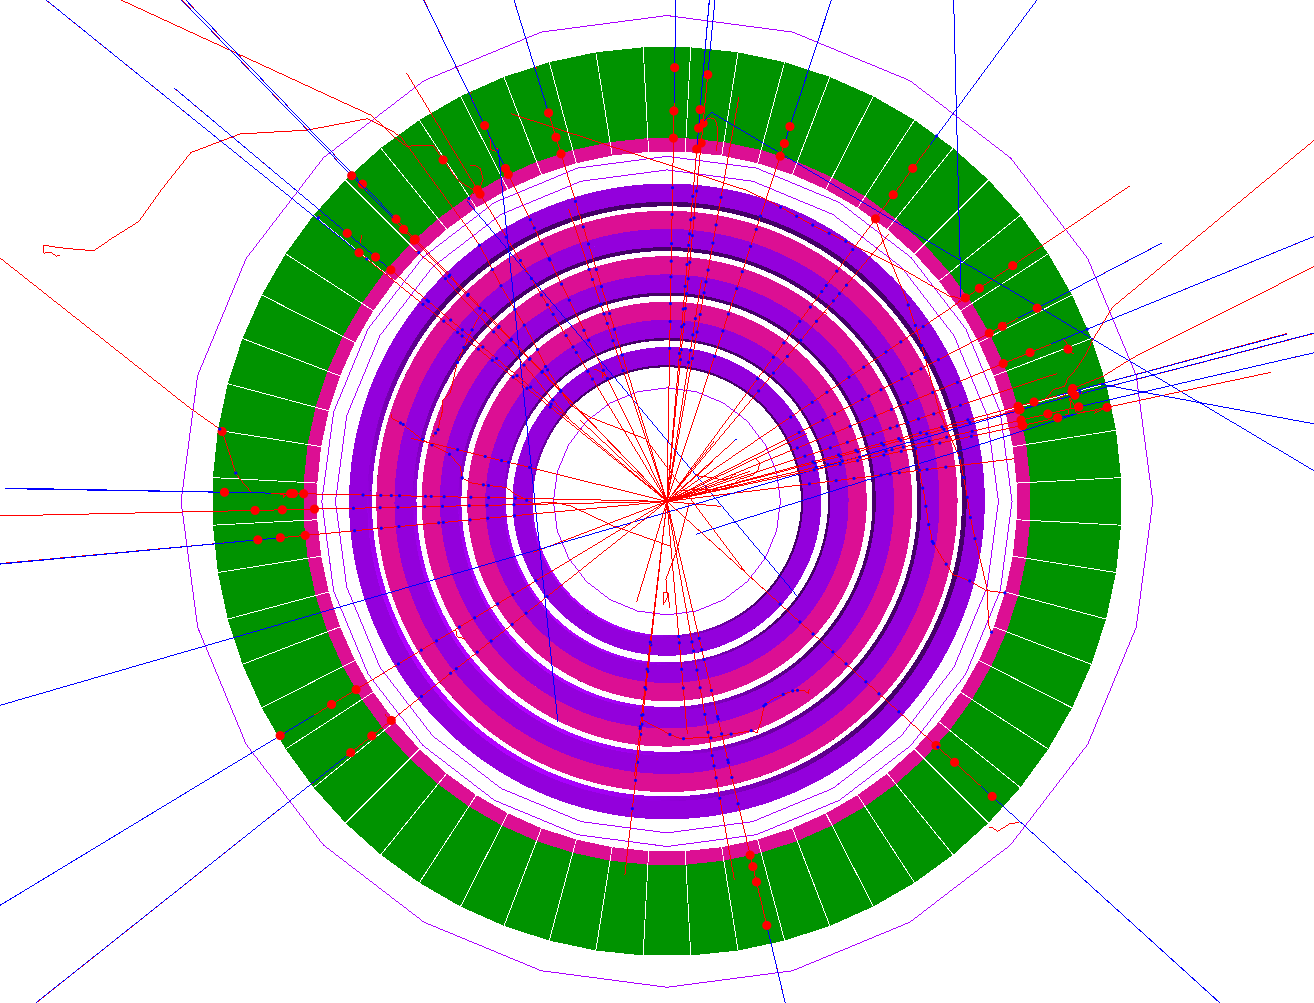
\includegraphics[width=0.8\textwidth]{gemc_alert_face_withHits.png}
	\caption{\textit{GEMC} hits in ATOF and AHDC are visible as red and blue points.}
	\label{fig:alert_simu_example}
\end{figure}

Software developped for ALERT simulations is available here \url{...}